\section{Øvelse 8 - TCP/IP socket programming}

\subsection{Introduktion}
I denne øvelse i socket programmering, laves en TCP client og TCP server. Vi har valgt at programmere i det objektorienterede sprog C\#. Clienten skal kunne forbinde til serveren, og downloade en fil herfra. Clienten og serveren køres på hver sin virtuelle linux maskine. I dette dokument beskrives udviklingsforløbet med tilhørende digrammer og kodeforklaringer.
\subsection{Udviklingsforløb}
Vi har designet koden således at server og client er opdelt i to hoveddele, hhv. constructor og overføringsfunktionalitet. For serveren betyder dette afsendingsfunktionalitet, og for clienten modtagelsesfunktionalitet.

\begin{lstlisting}[caption = Hoveddesign for server,label=herp]
public FileServer()
{
	//Setting up server and connecting client
	//Getting filename an calculating lenght
	//Sending file 
	//Closing connection
}
public void SendFile(string filename, long filesize, NetworkStream stream)
{
	//Local variables
	//Assigning variables
	//Sending file
	//Closing connection
}
\end{lstlisting}

\subsection{Funktionalitet}
Vores design gør det muligt for brugeren at selv indtaste en ønsket TCP servers IP-addresse. Dette giver mulighed for yderligere udvidelse af programmets funktionalitet. Der oprettes nu forbindelse til serveren med den indtastede addresse. Herefter venter clienten på at brugeren indtaster et navn på den fil der ønskes downloadet fra serveren. Clienten  anmoder da serveren om den specifikke fil, hvorefter serveren melder tilbage. Hvis filen eksisterer påbegyndes overførslen.

\subsection{Resultater}

\begin{figure}[h]
	\centering
	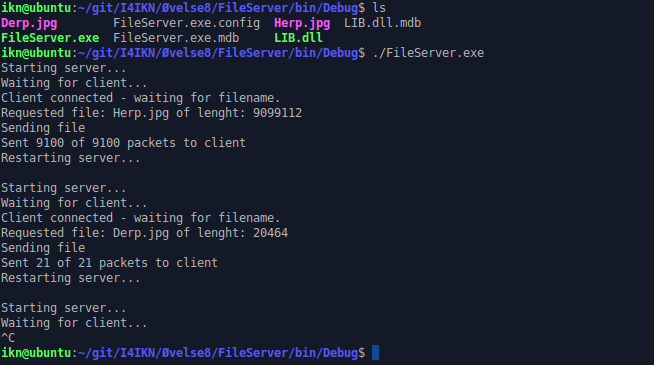
\includegraphics[width=0.9\linewidth]{figs/tcp_h1}
	\caption{Test af TCP server/client - billede fra server.}
	\label{fig:tcp_h1}
\end{figure}

\begin{figure}[h]
	\centering
	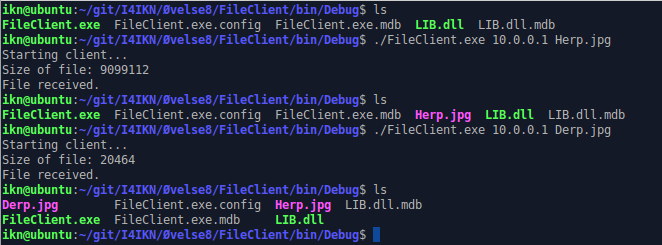
\includegraphics[width=0.9\linewidth]{figs/tcp_h2}
	\caption{Test af TCP server/client - billede fra client.}
	\label{fig:tcp_h2}
\end{figure}

\subsection{Konklusion}
I arbejdet med TCP socket programmering er vi kommet frem til en læsning der opfylder kravene givet i opgaven. Det kan derfor konstateres at teorien stemmer overens med praksis.